\chapter{Introduction}
\label{chap:intro}
\chaptermark{Introduction}

Worldwide electricity generation from non-hydroelectric renewable energy sources --- solar, wind, biomass, ethanol, and geothermal --- has grown considerably over the past several decades, increasing from 30 TWh in 1980 to almost 1,692 TWh in 2015~\cite{EIA2018a}. During this period of growth (see Figure~\ref{fig:gen-hist}), wind energy has played a leading role, increasing from 0.1 TWh in 1986 to over 833 TWh in 2015~\cite{EIA2018a}. Wind's exponential growth has been widespread, reaching, as a percent of total electricity generation, 9.8\% in the European Union (EU), 4.7\% in the United States (US), 3.3\% in China, and 1.5\% in the rest of the world~\cite{EIA2018a}. 

\begin{figure}[h!]
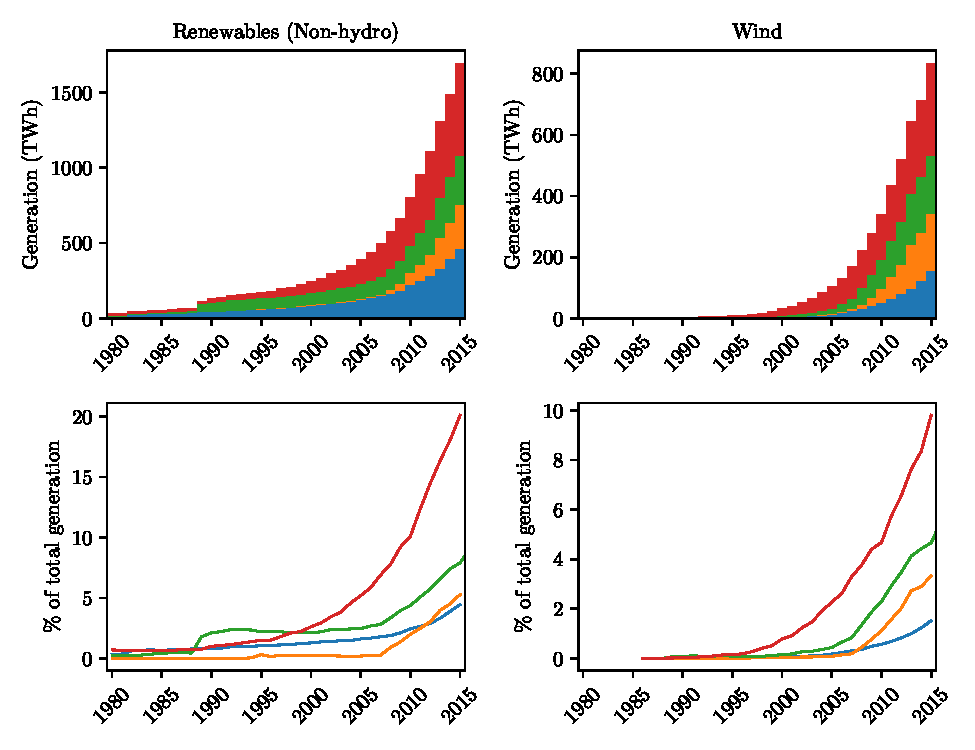
\includegraphics[width=\textwidth]{./wind-growth/gen-hist.pdf}
\caption{Growth in worldwide non-hydroelectric renewable electricity generation (left panels) and wind electricity generation (right panels). Renewable and wind generation are shown in TWh in the top panels and as a percentage of total generation in the bottom panels. Worldwide totals are displayed for the European Union ({\color{MPLred}\full}), United States ({\color{MPLgreen}\full}), China ({\color{MPLorange}\full}), and the rest of the world ({\color{MPLblue}\full}). Data from EIA~\cite{EIA2018a}.}
\label{fig:gen-hist}
\end{figure}

Wind's growth has not been uniformly distributed across the US and EU, with certain regions making significantly larger gains than other areas. In the EU, wind energy has reached nearly 50\% of total generation in Denmark, over 20\% in Ireland, Portugal, the Netherlands, and Lithuania, 18\% in Spain, and 13\% in Germany and the United Kingdom~\cite{EIA2018a}. In the US, wind generation is over 12\% of total generation in 11 states, including 31\% in Iowa and 25\% in South Dakota~\cite{GWEC2016a}.

The growth trends of wind have been driven by reduced costs and larger wind turbines. In the US, the levelized cost of energy for land-based wind has plummeted from nearly 600/MWh in 1980 to less than 50/MWh in 2015, and wind turbine rotor diameters and hub heights have increased from 17 m to over 100 m~\cite{DOE2015a}. As importantly, the environmental benefits of the move to wind energy are considerable. In the US, wind has reduced annual carbon dioxide emissions by 115,000,000 metric tons, sulfur dioxide emissions by 157,000 metric tons, nitrogen dioxide emissions by 97,000 metric tons, and water consumption by 36.5 billion gallons~\cite{DOE2015a}.

Wind energy's remarkable growth is expected to continue in the coming decades. The Global Wind Energy Center projects that wind will reach 15--40\% of global electricity demand by 2050, depending on future policy decisions~\cite{GWEC2016a}. In the US, the Department of Energy projects wind energy generation reaching 25\% of total demand by 2050 under 2015 policies with the potential to reach 35\% under more favorable policies~\cite{DOE2015a}.

\section{A challenge for grid integration of wind: Frequency regulation}
\label{sec:intro-freq-reg}
The continuing growth of variable and nondispatchable resources like wind energy has significant implications for the electric power system and will require changes in wind plant design and control. Over the last several years, wind has been operated as a niche energy source and grid operators have treated wind energy as a ``must take'' resource~\cite{Gil2013a}. As a result, wind plants prioritized maximizing power production because they were paid for every unit of power they produced. With growing grid penetration, however, wind energy has a growing potential to affect the overall state of the grid. A particular challenge for reliable power system operations under increased wind generation are ancillary services that maintain the stability of the grid~\cite{DOE2015a}. This has led grid operators and regulators to start requiring wind plants to participate in many of these services~\cite{Aho2012a, DiazGonzalez2014a}. 

Frequency regulation, which keeps the grid operating around its nominal frequency rating, is a particularly important ancillary service. Power systems currently rely on conventional dispatchable power sources to provide frequency regulation through short-term balancing of active power generation and load. As variable resources displace conventional generation, the resulting concern about the future availability of sufficient regulation participation has led many grid operators to consider expanding the pool of participating resources to include unconventional resources like wind energy~\cite{Aho2012a, DiazGonzalez2014a}. However, enabling full wind energy participation in frequency regulation involves many technological and economic challenges. A successful strategy will require new control designs that focus on power tracking rather than maximizing power output~\cite{Aho2012a}, modified frequency regulation market structures~\cite{Ela2014a, Ela2014b, Ela2014c}, expanded interconnection requirements for wind farms~\cite{Aho2012a, DiazGonzalez2014a}, and consideration of economic trade-offs between bulk power supply payments, ancillary service payments, and possible coordination with energy storage technologies~\cite{Rose2014a, Kirby2010a, DiazGonzalez2015a, Sun2010a}. 

Frequency regulation services act over many time scales to limit the deviation of the grid frequency from its nominal operating value in response to a grid disturbance, such as the failure of a major power plant of power transmission line. These services are classified into four categories of service, which each operate over a distinct time scale and serve a specific function. Figure~\ref{fig:freq-reg} shows the response of the grid frequency after a major generation loss and the time scales of each regulation service category.

\begin{figure}[h]
\begin{center}
\subimport{./fig/}{freq_reg.pdf_tex}
\end{center}
\caption{Response of power grid frequency to a major generation loss and the time scales of each regulation service category. Figure adapted from Aho \textit{et al.}~\cite{Aho2012a}.}
\label{fig:freq-reg}
\end{figure}

After a grid disturbance, inertial regulation acts instantaneously to limit the rate of frequency change and the maximum frequency deviation that occurs within several seconds. Primary regulation (droop control) acts over many seconds to drive the grid frequency towards a new steady-state operating value. Secondary regulation (automatic generator control) restores the system to its nominal frequency value by commanding participating generators to follow a power signal set by the grid operator over tens of minutes. Finally, tertiary regulation involves manually redistributing generation resources to restore normal operating conditions over several hours~\cite{Aho2012a, Rebours2007a, Rebours2007b}. 

Frequency regulation strategies using wind energy have focused on the first three regulation services because tertiary services occur over long time scales during which wind energy is too variable to provide balancing services. Instead, tertiary regulation is addressed through better scheduling, unit commitment, forecasting, or transmission system expansion~\cite{DOE2008a}. Combined inertial and primary regulation controls using wind turbines have been quite successful~\cite{Holdsworth2004a, Almeida2007a, Ma2010a, Morren2006a, Erlich2010a, Miller2011a, Hansen2014a}, even reducing the maximum and settling frequency deviation more effectively than traditional generators~\cite{Miller2011a, Gevorgian2015a}. Since aerodynamic interactions between turbines are relatively unimportant at time scales of less than a minute, combined inertial/primary controls can be implemented at the turbine level. 

With the success of inertial and primary frequency regulation control strategies, recent studies have begun to focus on secondary regulation~\cite{Buckspan2012a, Buckspan2013a, Aho2013a, Aho2014a, Jeong2014a, vanWingerden2017a, Boersma2017a}. Power plants participating in secondary frequency regulation typically provide power in both the bulk power market and the regulation market. The bulk power is supplied at some fixed level $P_0$ and the regulation service entails providing $\Delta P$ of regulation power that is controlled by the grid operator through the normalized regulation signal $r(t)$. The combined reference signal the plant must track is
\begin{equation}
P_\text{ref}(t) = P_0 + \Delta P \, r(t).
\end{equation}
Two example secondary regulation signals from PJM, a grid operator in the US that includes Baltimore, Maryland within its operating territory, are shown in Figure~\ref{fig:pjm}. As seen in these signals, the regulation signals vary on time scales on the order of minutes.

\begin{figure}[h]
\begin{center}
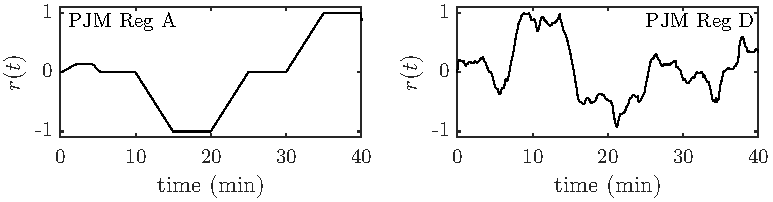
\includegraphics[width=\textwidth]{./fig/pjm.pdf}
\end{center}
\caption{Regulation signals from PJM~\cite{PJMm11, PJM2018a}, which has two regulation markets "RegA" and "RegD".}
\label{fig:pjm}
\end{figure}

A stand-alone turbine can regulate its instantaneous power output level through pitch and/or generator torque control, which enables it to follow a secondary regulation signal. While current wind turbine controllers operate at the maximum power point $P_*$, participation in the secondary frequency regulation market --- which includes increased power demand over the bulk power setpoint --- requires a wind turbine to reduce the amount of power it provides to the bulk power market~\cite{Aho2012a, Rose2014a, Kirby2010a, Aho2013a, Jeong2014a, Fleming2016a}. A particularly effective approach~\cite{Aho2013a} is to modify the generator torque control law such that the turbine operates at a higher-than-optimal tip speed ratio, thereby storing energy in the rotating rotor. Since a single wind turbine cannot provide power production greater than the maximum power point for an extended period, the derated generation setpoint is the maximum power point minus the regulation power; i.e. $P_0 = P_* - \Delta P$. This procedure is known as derating the turbine's power output. 

As a result, wind energy suppliers must consider the trade-offs between lost bulk power supply payments and additional ancillary service payments~\cite{Rose2014a, Kirby2010a}. Rose \& Apt~\cite{Rose2014a} found that these economic tradeoffs mean that given the current energy market design wind turbines can only provide secondary regulation more cost effectively that conventional generators less than 1\% of the time. This lack of profitability for providing regulation is because the secondary regulation price in competitive markets is equal to the lowest opportunity cost for a generator to provide regulation. This opportunity cost is the wholesale price of electricity less the generator's marginal cost that is dominated by fuel costs. A conventional generator's marginal cost is a significant fraction of the wholesale electricity price and a wind plant has a near zero marginal cost because wind is free~\cite{Rose2014a}. Therefore, wind energy is unlikely to have a lower opportunity cost than conventional generators. Kirby \textit{et al.}~\cite{Kirby2010a} found similar tradeoffs, but noted that in cases of high wind generation, conventional generators are forced to pay high costs related to minimum loads and regulation prices remain relatively stable. This makes wind energy cost competitive during some time periods~\cite{Kirby2010a}. Rose and Apt~\cite{Rose2014a} also note that the cost of developing secondary regulation controllers is low and should be required as an additional grid stability contingency. 

\section{Providing secondary frequency regulation with wind farms}
\label{sec:intro-secondary-wind}
In addition to the economic challenges outlined above, applying the single-turbine approach to wind farms is not straightforward because aerodynamic interactions between turbines complicate controlling the power output of an entire farm. Wind turbines in a farm are aerodynamically coupled by wakes, which are regions of reduced velocity and increased turbulence behind the turbines, depicted by the fog shown in Figure~\ref{fig:wind_farm_wake}. Control actions at an individual wind turbine modify the strength and characteristics of the wake behind the rotor, which in turn affects the subsequent power production of downstream turbines as the wake travels downwind and interacts with wakes of subsequent and adjacent turbines. In large wind farms, this complicated aerodynamic coupling is unavoidable. Wind turbine wakes extent tens of rotor diameters downstream, and moving downstream turbines away from the wakes of upstream turbines is impossible in practice given space constraints.

Several aerodynamic control variables can affect wind farm power output in a dynamic and coupled manner. Thrust modulation through pitch or generator torque control~\cite{Annoni2015b} affects the magnitude of the velocity behind the wake. Yawing, where the turbine is misaligned with the incoming wind direction, can redirect wakes toward or away from downstream turbines~\cite{Fleming2014a, Fleming2015a}. Tilting of the rotor can also dynamically affect wind farm power by redirecting wakes and modifying the entrainment of kinetic energy~\cite{Fleming2014a, Verhulst2015a, Annoni2017a}.

For example, suppose thrust modulation is employed at a turbine at the beginning of the farm. If the turbine pitches its blades from a feathered configuration toward the optimal pitch angle, the power generation at that turbine will increase and the velocity in the turbine's wake will be reduced. As a result, the generation of downstream turbines will decrease, but only after the wake has traveled to the downstream turbine. This complex and time-varying aerodynamic coupling of upstream turbine control actions and downstream turbine power generation is a particular challenge for secondary frequency regulation because the travel time of the wind from one turbine to the next and the time it takes the wind to travel the length of the farm is routinely the same or longer than the duration and frequency of typical regulation signals.

\begin{figure}[h]
\begin{center}
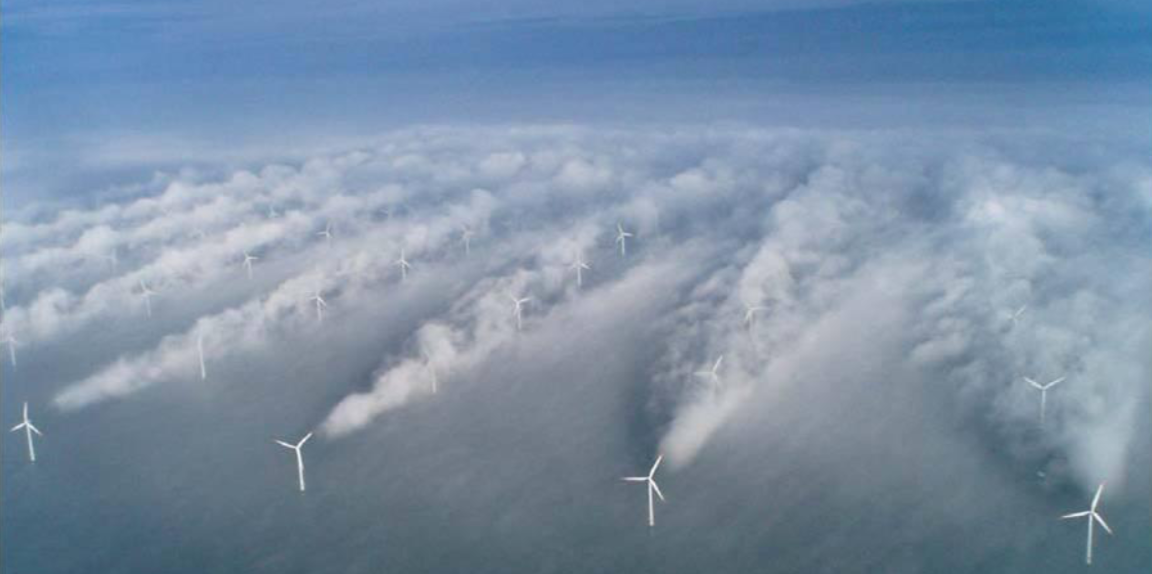
\includegraphics[width=\textwidth]{./fig/wind_farm.png}
\end{center}
\caption{Wind turbine wakes in Horns Rev wind farm visualized by the formation of fog. Figure is reproduced from Hasager \textit{et al.}~\cite{Hasager2013a} and licensed under CC BY 3.0.}
\label{fig:wind_farm_wake}
\end{figure}

Clearly, providing secondary regulation for the power grid with wind farms is more complicated than the single turbine case. Issues have been demonstrated in numerical simulations of a wind farm where each wind turbine employs a tracking method that neglects aerodynamic interactions~\cite{Fleming2016a}. When downstream turbines were placed away from upstream wakes, the farm was able to track the secondary frequency regulation signal. However, when downstream turbines were placed in the wakes of upstream turbines, the tracking performance of the downstream turbines was significantly degraded. 

One successful single-turbine approach was a proportional-integral controller that employs the same single-turbine control strategy but compensates for underperforming turbines by increasing the power production of other turbines operating below the maximum power point~\cite{vanWingerden2017a}. The resulting closed-loop wind farm provides good tracking performance in tests employing high-fidelity simulations as a wind farm model. However, the derate used~\cite{vanWingerden2017a} was larger than the regulation power, sacrificing considerable revenue in the bulk power market. As a result, approaches that do not consider interactions between turbine wakes~\cite{Hansen2006a, Hansen2006b} or use steady-state wake models that ignore the time-varying nature of these interactions~\cite{Ahmadyar2015a, Badihi2015a} may be unable to provide secondary frequency regulation. Ultimately, given the complexity of the aerodynamic interactions between turbines, more work is needed to develop effective controls for secondary frequency regulation. 

\section{Wind farm models and control}
\label{sec:intro-models}
Wind farm control designs have generally relied on model-based approaches to address the complexity of wind farm aerodynamics. Available wind farm models vary tremendously in complexity and accuracy. Static wake models have played a leading role in wind farm design for decades. The Jensen model~\cite{Jensen1983a, Katic1986a} treats the initial wake as a top-hat profile with an initial deficit specified using actuator disk theory~\cite{Burton2011a} and assumes that the diameter of the wake expands linearly with downstream distance through turbulent mixing, as shown in Figure~\ref{fig:jensen}. Other wake-centric models have mirrored this approach~\cite{Ainslie1988a, Bastankhah2014a, Niayifar2015a, Niayifar2016a, Archer2018a, Frandsen2006a, Gebraad2014c}. Top-down models~\cite{Frandsen1992a, Frandsen2006a, Calaf2010a, Meneveau2012a} view the wind farm as an added roughness that affects the entrainment of kinetic energy from above. Stevens~\textit{et al.}~\cite{Stevens2015a, Stevens2016c} recently coupled these two approaches to improve the results.

\begin{figure}[h]
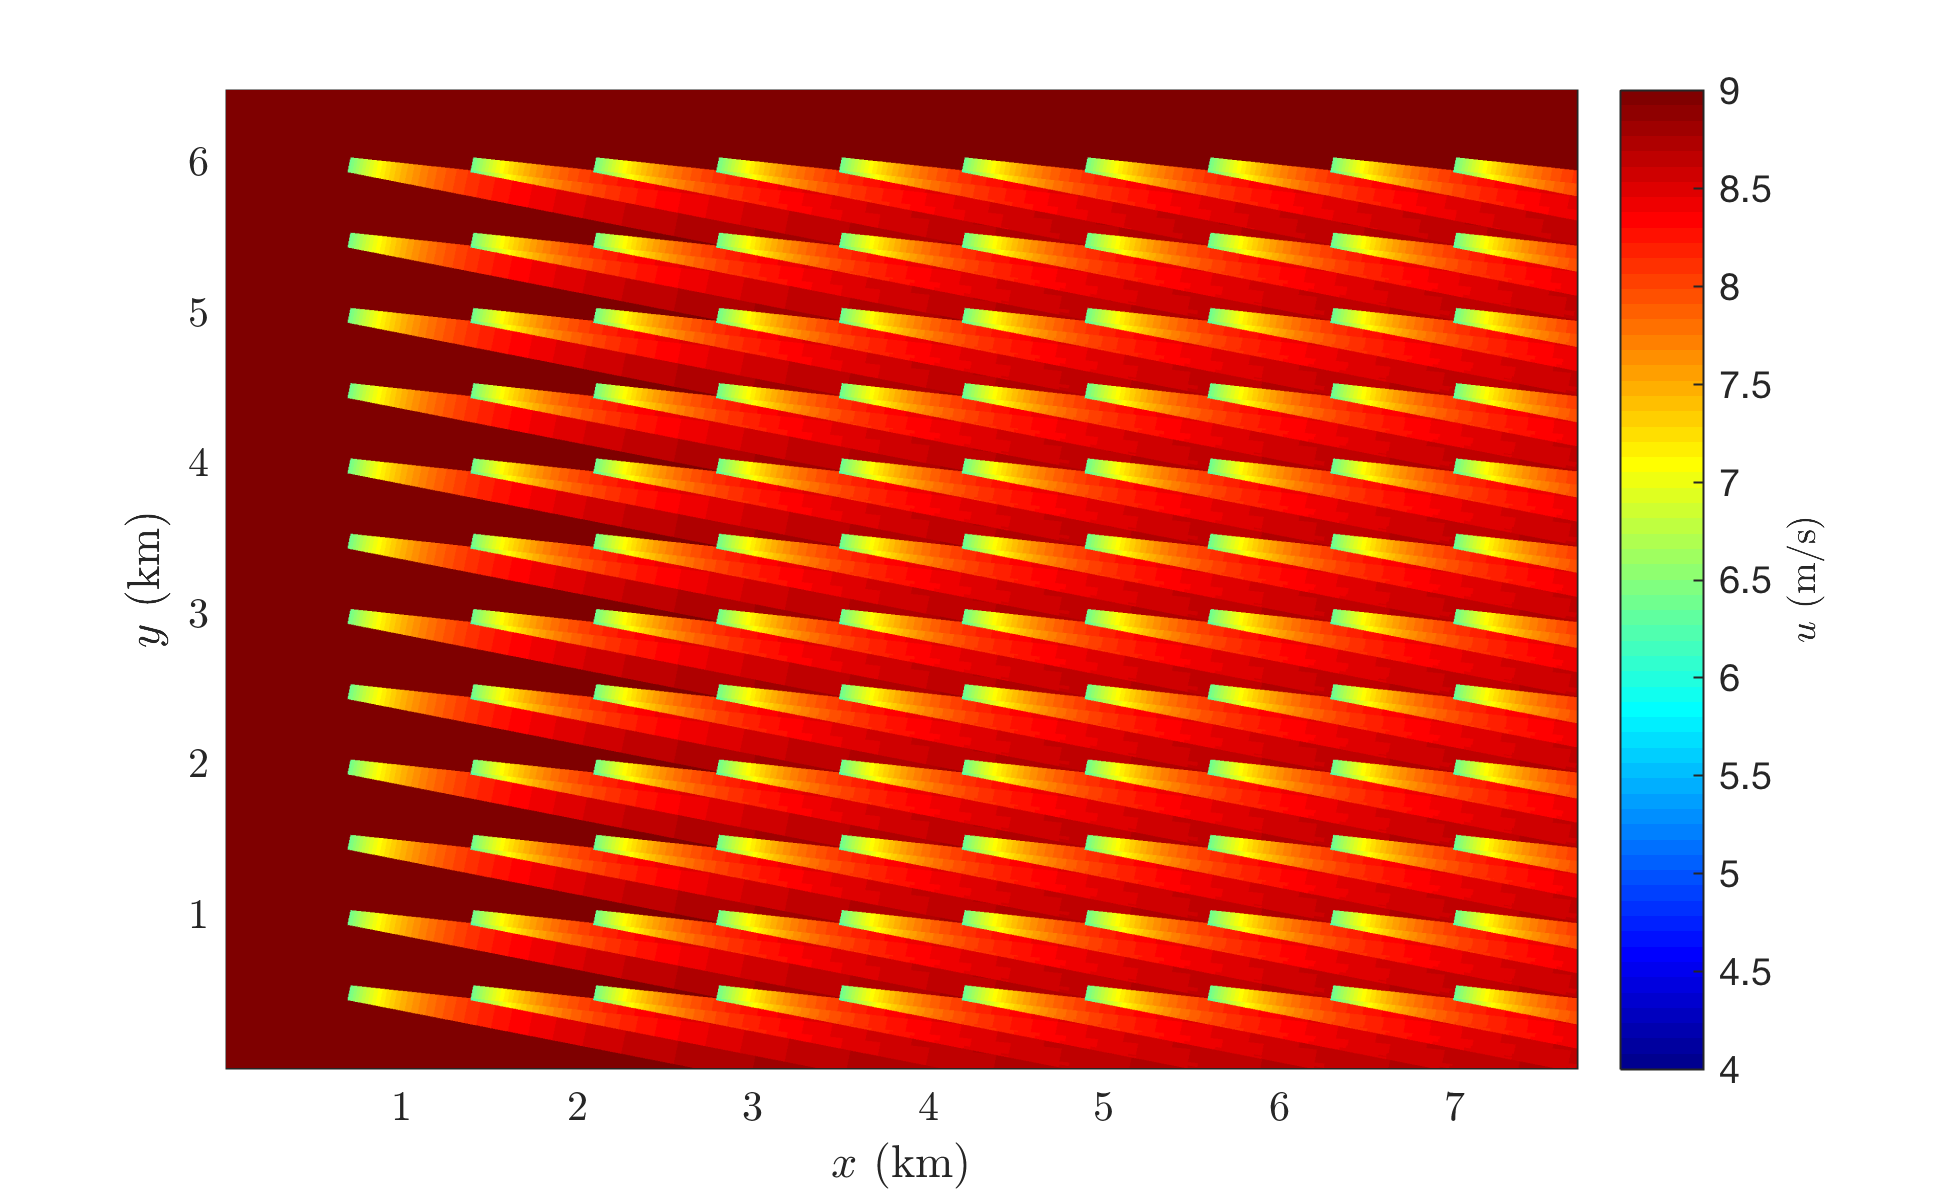
\includegraphics[width=\textwidth]{./fig/jensen.png}
\caption{Jensen model of a wind farm with 120 turbines with an inflow of $U_\infty = 9$ m/s.}
\label{fig:jensen}
\end{figure}

These static wake models, however, are unable to model yawed and tilted turbines. Wake models that account for these effects, unfortunately, have not been as successful in predicting wind farm behavior. Most notably, momentum balance arguments~\cite{Burton2011a, Jimenez2010a}, Glauert's proposed equation for the axial induced velocity through the rotor~\cite{Glauert1926a}, and the skewed elliptic vortex cylinder model~\cite{Coleman1945a, Branlard2016a} lead to conflicting results that do not always agree with simulations of yawed wind farms. Resolving the significant differences among these models is vital for providing secondary frequency regulation control with yawing or tilting.

Although static wake models have improved wind farm design and analysis, these models lack dynamics to model the effects of time-dependent changes in thrust coefficients and other operating conditions in general. In recent years, dynamic models have been proposed that account for the movement of wakes through the wind farm as well as turbulent mixing of wakes with the surrounding air through extensions of the classic Jensen wake model~\cite{Larsen2008a, Annoni2016b, Gebraad2014b, Gebraad2015b}. Higher-fidelity approaches include input-output dynamic mode decomposition~\cite{Annoni2016a}, the restricted nonlinear model~\cite{Bretheim2018a}, and the two-dimensional Navier-Stokes equations~\cite{Doekemeijer2017a, Boersma2018a}. Despite these advances, fully functioning wind farm controllers have yet to be built around these dynamic modeling approaches.

Control designs using high-fidelity simulations have been used successfully for similar problems, including drag reduction in turbulent boundary layers~\cite{Bewley2001a} and power maximization of wind farms~\cite{Goit2015a}. In these studies, numerical simulations of the flow states of these systems were taken as state-space representations, and control trajectories were determined by solving an online optimization problem using adjoint-based gradient methods. While this approach could also be applied to the secondary frequency regulation power tracking problem, the size of the optimization problem is too large to be solved in real time in any foreseeable future~\cite{Goit2015a}. 

\section{Outline}
\label{sec:intro-outline}
This thesis works towards a unified control framework for power tracking with wind farms using thrust and yaw modulation. Furthermore, we aim to reduce the derate requirements for wind farms providing secondary frequency regulation by storing energy in the wind flow field or the rotation of the rotor.  (See Appendix~\ref{app} for estimates of energy storage potential). This project includes (1) building dynamic wake models that account for the physics of wake advection, wake expansion through turbulent mixing, and wake deflection through yaw; (2) developing sensing and estimation tools to correct modeling errors using measurements from wind farms; and (3) developing controllers to provide power tracking with the error corrected models. The rest of this thesis is organized into the following chapters.

In Chapter~\ref{chap:methods}, we discuss the methods and tools used to develop and evaluate wind farm controls, including large eddy simulations and optimal control of PDE systems. In Chapter~\ref{chap:dynwake}, a dynamic wake model is presented that includes wake advection and expansion. A lifting line approach is used in Chapter~\ref{chap:yaw} to develop wake models that accurately predict the deflection of wakes behind yawed turbines. Sensing and estimation methods for the dynamic wake model are discussed in Chapter~\ref{chap:estimation}. Chapter~\ref{chap:rhc} presents the model-based receding horizon controller used to provide secondary frequency regulation and evaluates the control method using grid operator performance metrics and compares the control to a controller build around a static model. Chapter~\ref{chap:rhc2} discusses extensions of the controller presented in Chapter~\ref{chap:rhc} to allow for arbitrary wind farm configurations and incorporate rotor dynamics and inertia as well as realistic wind farm control variables. Conclusions and future work are discussed in Chapter~\ref{chap:conclusions}.